%%%%% Beginning of preamble %%%%%
\documentclass[12pt]{article} 

%What kind of document (article) and what size
%Packages to load which give you useful commands
\usepackage{amssymb, amsmath, amsthm} 
\usepackage{epsfig,graphicx} 
\usepackage{caption}
\usepackage{subcaption}
\usepackage{multirow}

%Sets the margins
\textwidth = 6.5 in 
\textheight = 9 in 
\oddsidemargin = 0.0 in 
\evensidemargin = 0.0 in 
\topmargin = 0.0 in 
\headheight = 0.0 in 
\headsep = 0.0 in \parskip = 0.2in \parindent = 0.0in

\begin{document} 

\section{Communities Detection}

In order to test our hypothesis we ran a community detection algorithm on the two networks under analysis: the one produced by the toy model and the Twitter one. 
We used the algorithm developed by Blondel at al. \cite{blondel2008fast}, which is found to be one of the best algorithms for community detection based on modularity 
optimization, as shown by Fortunato in his review of communities detection methods\cite{fortunato2010community}. 
The algorithm works in two phases: in the first one the modularity is optimized by allowing only local changes of communities, 
and in the second one the found communities are aggregated in order to build a new network of communities. 
These two phases are repeated iteratively until no increase of modularity is possible.
In the future we plan to expand the analysis by using also other algorithms, such as Infomap\cite{rosvall2010mapping}, and compare the obtained results.
The analysis was carried out in two steps: first we applied the algorithm to the binary unweighted network, considering in this way only the \textit{structural}
relationships between the nodes. These are given, in the case of the real data, by looking at who is \textit{following} who on Twitter, which is an
explicitly declared relationship. The limitation of this method is that most Twitter users follow a very large number of people, but in practice they
see and share only the tweets belonging to a relatively small subset of the users they follow. Therefore the second step was to apply the algorithm 
to a weighted version of the networks, that we obtained by weighting each structural link with the value of the mutual information between the two users.
The results of this analysis are shown in Table~\ref{table_modularity}.

\begin{center}
\begin{table}[!ht]
\begin{tabular}{c|c|c|c|c|}
\cline{2-5}
& \multicolumn{2}{|c|}{Synthetic Network} & \multicolumn{2}{|c|}{Twitter Network} \\ \cline{2-5}
& Binary & Weighted & Binary & Weighted \\ \cline{1-5}
\multicolumn{1}{ |c| }{Number of Detected Communities} & 8 & 4 & 26 & 37 \\ \cline{1-5}
\multicolumn{1}{ |c| }{Optimal Modularity Value} & 0.264 & 0.625 & 0.260 & 0.404 \\ \cline{1-5}
\end{tabular}
\caption{Communities Detection Results}
\label{table_modularity}
\end{table}
\end{center}

We can observe a clear increase in the optimal value of modularity when we consider the weighted network, which indicates that the network has a more
defined community structure. In the case of synthetic data the value triples, whereas in the case of real data it doubles. This result shows, as we expected,
that if we weight the structural links of a network with a measure of the communication flow among the nodes, giving thus more importance to the links
between two users that actually share information and less to the links that are there but are not exploited, we can detect a finer community structure.
In particular, for what concerns the synthetic data, we can observe that in the weighted case we find exactly four communities, which is coherent to the way
the toy model was built. A visual representation of the results is given in Figure~\ref{networks_synthetic} for the synthetic data and in 
Figure~\ref{networks_twitter} for the Twitter data.

\begin{figure}[!ht]
\centering
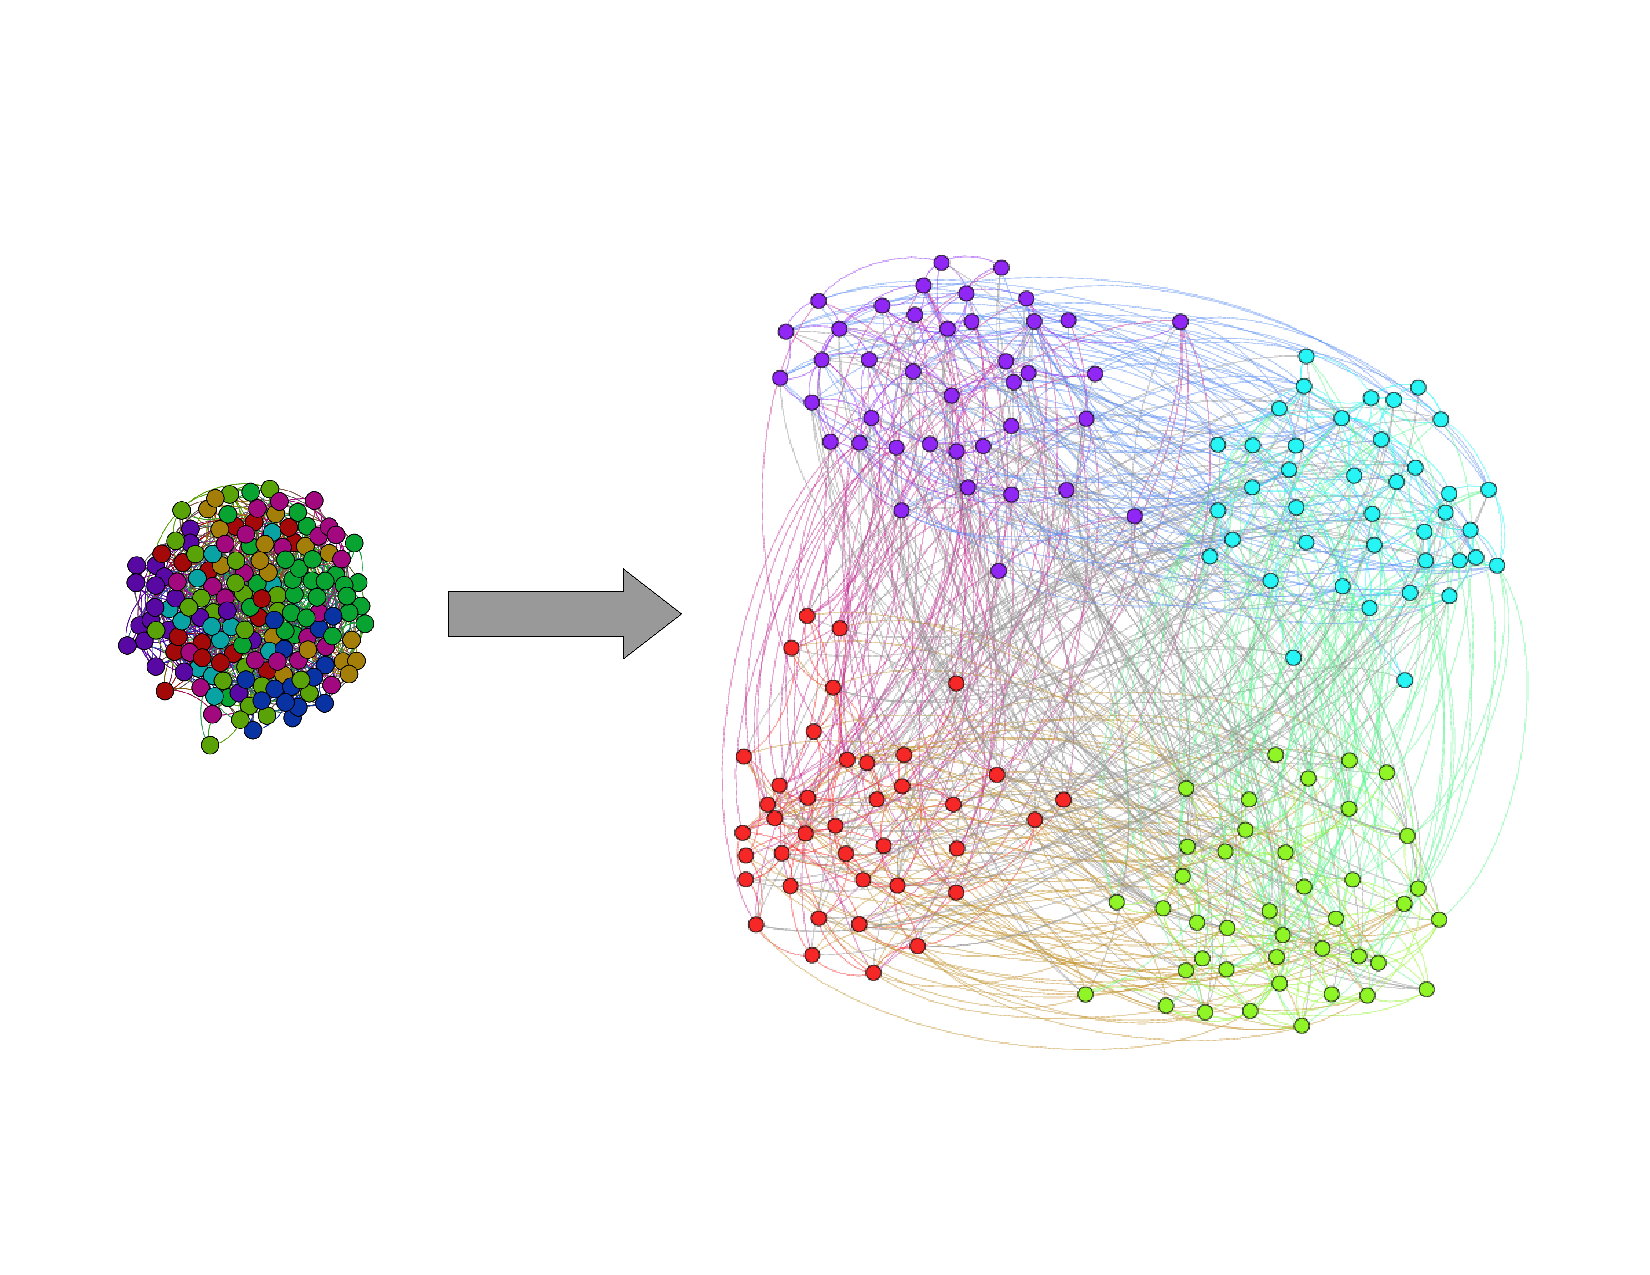
\includegraphics[width=0.72\textwidth]{Figures/synthetic_data_networks.pdf}
\caption{Visualisation of the synthetic network obtained using binary edges (left figure) and weighted ones (right figure). Node colors indicate the
community affiliation.}
\label{networks_synthetic}
\end{figure}

\begin{figure}[!ht]
\centering
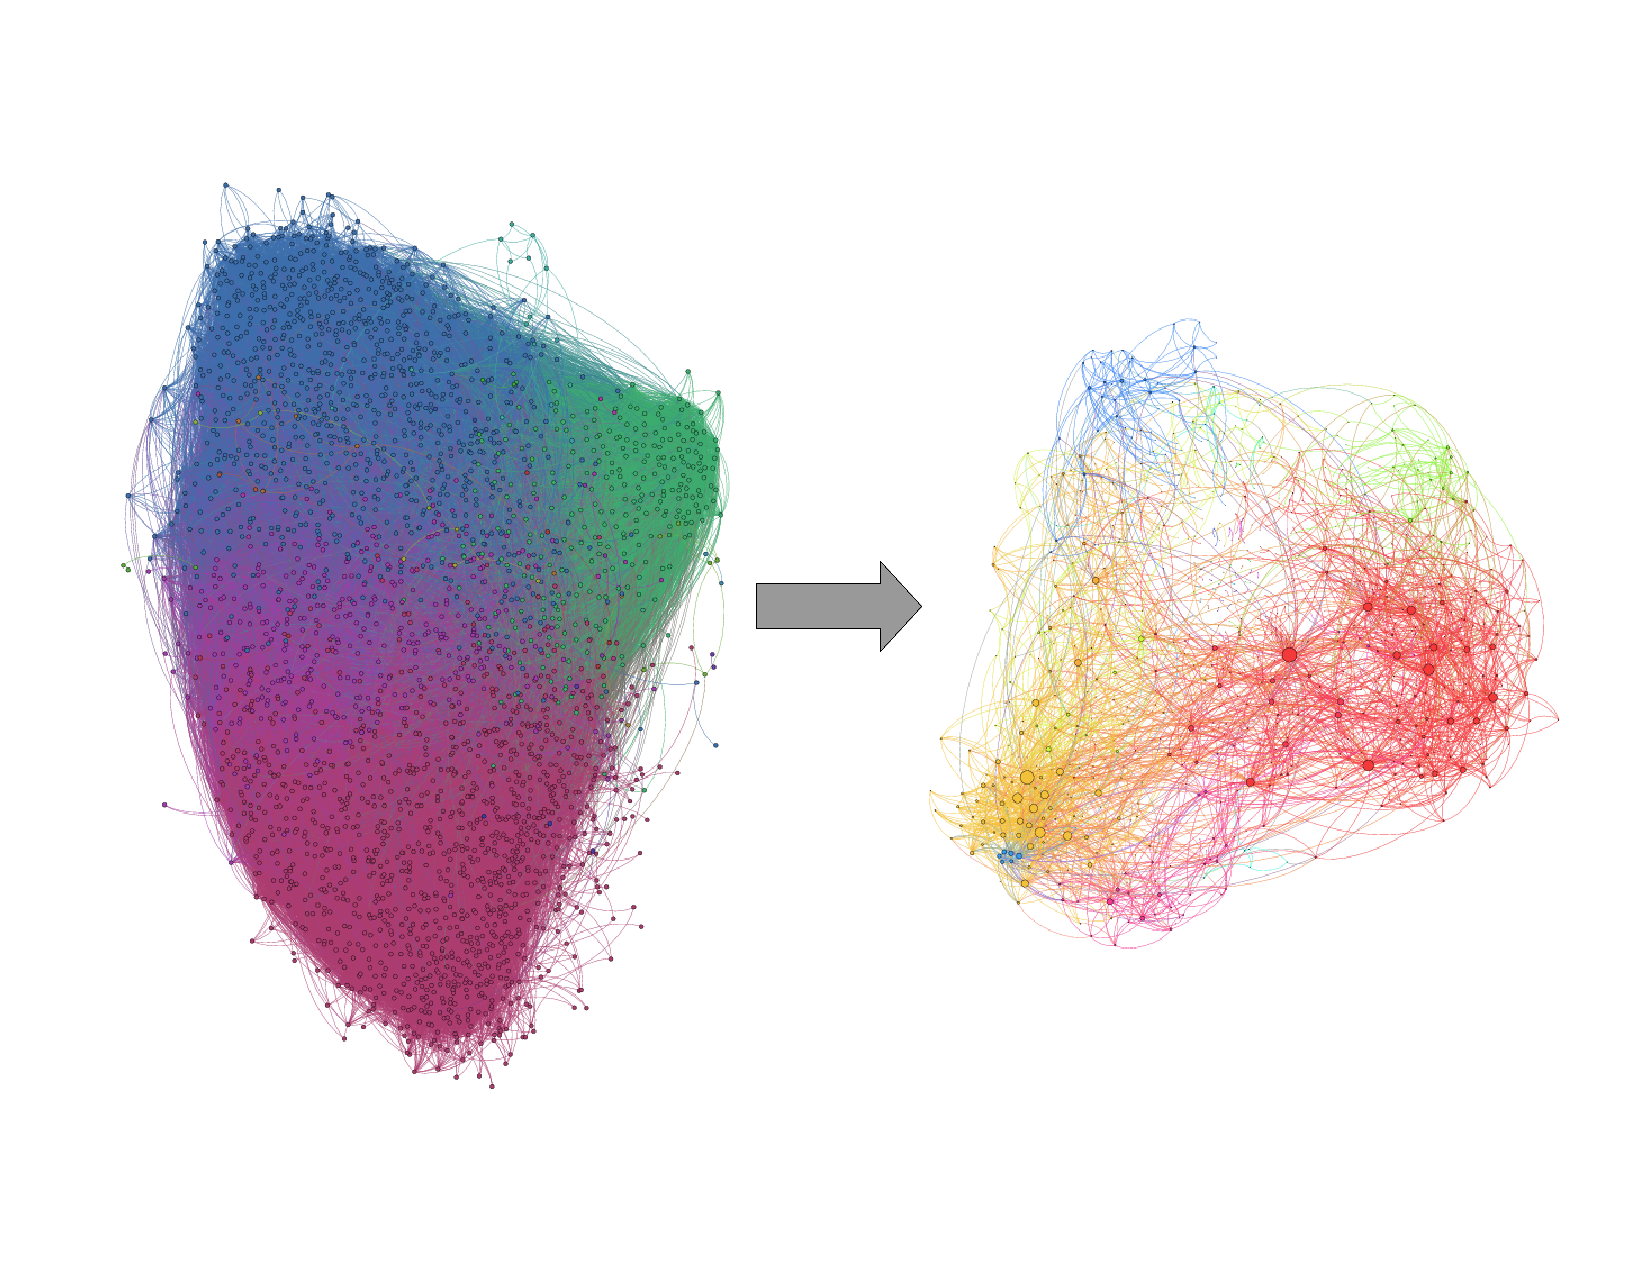
\includegraphics[width=0.72\textwidth]{Figures/twitter_data_networks.pdf}
\caption{Visualisation of the Twitter network obtained using binary edges (left figure) and weighted ones (right figure). Node colors indicate the
community affiliation.}
\label{networks_twitter}
\end{figure}

\section{Sanity Check}
Dave, could you please take care of this part since it's you who worked on that?

\bibliographystyle{plain}
\bibliography{../references}

\end{document}
